%%% File encoding: UTF-8
%% äöüÄÖÜß  <-- no German Umlauts here? Use an UTF-8 compatible editor!

%%% Magic comments for setting the correct parameters in compatible IDEs
% !TeX encoding = utf8
% !TeX program = pdflatex 
% !TeX spellcheck = en_US
% !BIB program = biber

\documentclass[master,english]{hgbthesis}
% Permissible options in [..]: 
%   Type of work: diploma, master (default), bachelor, internship 
%   Main language: german, english (default)
%%%----------------------------------------------------------

\RequirePackage[utf8]{inputenc}		% Remove when using lualatex or xelatex entfernen!
\usepackage{graphicx}
\usepackage{svg}
\usepackage{minted}
\usepackage{listings}
\usepackage{varioref}
\usepackage{longtable}
\usepackage{tabularx}

% -----------------------------------------------------
\newenvironment{code}{\captionsetup{type=listing}}{}
% -----------------------------------------------------
% -----------------------------------------------------
\newcommand{\mysubsubsection}[1]{{\subsubsection{\textbf{#1}}}}
\newcommand{\mentionedtext}[1]{{\textit{{#1}}}}
\newcommand{\sourceDir}{./sources}
\newcommand{\sourceFontSize}{\fontsize{10pt}{11.5}}
\newcommand{\quotes}[1]{``#1''}
\newmintedfile[bashFile]{bash}{
	linenos=false, 
	frame=none, 
	breaklines=true, 
	tabsize=2,
	numbersep=5pt,
	xleftmargin=10pt,
	baselinestretch=1,
	fontsize=\sourceFontSize
}
\newmintedfile[yamlFile]{yaml}{
	linenos=false, 
	frame=none, 
	breaklines=true, 
	tabsize=2,
	numbersep=5pt,
	xleftmargin=10pt,
	baselinestretch=1,
	fontsize=\sourceFontSize
}
\newmintedfile[javaFile]{java}{
	linenos=false, 
	frame=none, 
	breaklines=true, 
	tabsize=2,
	numbersep=5pt,
	xleftmargin=10pt,
	baselinestretch=1,
	fontsize=\sourceFontSize
}
\newmintedfile[xmlFile]{xml}{
	breaklines=true, 
	tabsize=2,
	numbersep=5pt,
	xleftmargin=10pt,
	baselinestretch=1,
	autogobble=true,
	breakautoindent=false,
	fontsize=\sourceFontSize
}
\newmintinline[inlineJava]{java}{
	fontsize=\sourceFontSize
}
\newmintinline[inlineBash]{bash}{
	fontsize=\sourceFontSize
}
% -----------------------------------------------------
\graphicspath{{images/}}    % location of images and graphics
\logofile{logo}				% logo file = images/logo.pdf (use \logofile{} for no logo)
\bibliography{references.bib}  	% name of bibliography file (references.bib)
\setlength{\parindent}{0pt}

%%%----------------------------------------------------------
% Title page entries
%%%----------------------------------------------------------

%%% Entries for ALL types of work: --------------------------
\title{Implementation of an Enterprise Service Bus with OpenShift} %no camel used (and Camel)
%\author{Ing. Thomas Herzog B.Sc}
%\programname{Software Engineering}
\placeofstudy{Hagenberg}
\dateofsubmission{2018}{09}{17}	% {YYYY}{MM}{DD}

%%% Entries for Bachelor theses only: -----------------------
%\thesisnumber{XXXXXXXXXX-A}   %e.g. 1310238045-A  
% (Stud-ID, A = 1st Bachelor thesis)
%\semester{Fall Semester 2017} 	% Fall/Spring Semester YYYY
%\coursetitle{Introduction to Trivial Problems 1} 
\advisor{DI (FH) Peter Kulczycki}

%%% Restricted publication license instead of CC (master only):
\cclicense

%%%----------------------------------------------------------
\begin{document}
%%%----------------------------------------------------------

%%%----------------------------------------------------------
\frontmatter							% title part (roman page numbers)
%%%----------------------------------------------------------

\includepdf{title.pdf}
\maketitle
\tableofcontents

%\include{front/preface} 	% preface is optional
\chapter{Abstract}
An Enterprise Service Bus (ESB) is a crucial part of an enterprise, which connects the enterprise to its partners, customers, and other branches. The appearance of containerization, cloud services, and the microservice architecture have provided new possibilities for implementing and running an ESB. But, an ESB is commonly used by large conservative enterprises, which don't adapt new technologies fast, and wait until a new technology has proven itself. Especially the cloud is something the industry denied to use for a long time, because of the fact, that the infrastructure and data are managed and maintained by external service providers. \\ 

These days, we live in the so called cloud age, whereby global enterprises like Red Hat or Amazon provide cloud services such as Platform as a Service (PaaS), which can scale with the business. Enterprises start to consider to move their ESB installations to the cloud to profit from the cloud service provided features. Moving an ESB to the cloud will be a long term process for an enterprise, because the established processes for development, running, and managing the ESB will have to change. \\

This thesis has the goal to give the reader an overview of the cloud related concepts and technologies such as, Infrastructure as Code (IaC) and Docker, which are the base for cloud services. The implemented ESB prototype,  is  available at \url{https://github.com/cchet-thesis-msc/prototype}, and shows how an ESB could be implemented on a PaaS platform. \\




%%%----------------------------------------------------------
\mainmatter          			% main part (arabic page numbers)
%%%----------------------------------------------------------

\chapter{Introduction}
\label{cha:intro}

\section{Motivation}
\label{sec:intro-motivation}
Large enterprises work with several independent applications, where each application covers an aspect of a business of an enterprise. In general, these applications are from different vendors, implemented in different programming languages and with their own life cycle management. To provide a business value to the enterprise, these applications are connected via a network and part of a business workflow. The applications have to interexchange data, which is commonly represented in different data formats and versions. This leads to an highly heterogeneous network of applications, which is very hard to maintain.

The major challenge of an IT department is the integration of independent applications into the enterprise application environment. The concept of Enterprise Application Integration (EAI) provides patterns [\cite{EIP}], which help to define a process for the integration of applications into a heterogeneous enterprise application environment. One of these patterns is the Enterprise Service Bus (ESB), which is widely used in the industry.

Often the term ESB application is used to refer to an ESB, which connects multiple applications. But an ESB is a software architectural model, rather than an application. The term could have been established by the usage of middleware such as JBoss Fuse [\cite{Fuse2018}], which helps to integrate applications into an ESB. JBoss Fuse is based on the JBoss Enterprise Application Platform (JBoss EAP), where the applications are integrated in a existing runtime environment. 

With the upcoming of cloud solutions such as Platform as a Service (PaaS) [\cite[p. 2-3]{PaaS2015}] it is now possible to move the platform from a dedicated environment to a cloud environment, where the cloud provider will take over responsibility for maintenance and security of the platform. The concept of Integration Platform as a Service (IPaaS) [\cite[p. 3]{iPaaSP12015}] is on top of PaaS and enhances a common PaaS solution with the Integration features needed by EAI.
   
Thus, enterprises can now reduce the effort in implementing an ESB, integrating applications into the ESB and reducing the costs of of an ESB by using a consumption based pricing model.

\newpage
\section{Objectives}
\label{sec:intro-objectives}
This thesis aims to implement an ESB on Openshift PaaS [\cite{Openshift2018}]. Commonly an ESB is implemented with the help of middleware such as JBoss Fuse, which is based on the JBoss EAP. The concepts of PaaS and IPaaS in combination with an ESB are in general new to the industry. In general the industry hosts their ESBs in their own data centers, due to the lack of trust for cloud solutions. 

A main focus of this thesis is how applications internal and external can be integrated and managed in the PaaS solution Openshift. The different aspects of applications integrated into an ESB such as security, staging and versioning of will also be discussed in this thesis. The security is commonly managed by a middleware, which is in general hosted on a dedicated data center owned by the enterprise. With the usage of PaaS such as Openshift the responsibility of the security mostly shifts to the cloud provider.

// TODO: Futher writing
 




\chapter{Infrastructure as Code}
\label{cha:iac}
Infrastructure as Code (IaC) is a concept to automate system creation and change management with techniques from software development. Systems are defined in a Domain Specific Language (DSL), which gets interpreted by a tool, which creates an instance of the system or applies changes to it. IaC defines predefined, repeatable routines for managing systems \cite{Morris2016}. IaC descriptions are called templates, cookbooks, recipes or playbooks, depending on the tool. In the further course, the IaC definitions will be called templates. The DSL allows to define resources of a system such as network, storage and routing descriptively in a template. The DSL abstracts the developer from system specific settings and provides a way to define the system with as little configuration as possible. The term system is used as a general description. In the context of IaC, a system can be anything which can be described via a DSL.

\section{The Need for Infrastructure as Code}
\label{sec:iac-need}
In the so called iron age, the IT systems were bound the physical hardware and the setup of such a system and its change management were a long term, complex and error prone process. These days, we call such systems legacy systems. In the cloud age, the IT systems are decoupled from the physical hardware and in the case of PaaS they are even decoupled from the operating system \cite{Morris2016}. The IT systems are decoupled from the physical hardware and operating system, due to the fact, that cloud providers cannot allow their customer to tamper with the underlying system and hardware. In general, the hardware resources provided by a cloud provider are shared by multiple customers. \\

With IaC it is possible to work with so called Dynamic Infrastructure Platforms, which provide computing resources, where the developers are completely abstracted from the underlying system. Dynamic infrastructure platforms have the characteristic to be programmable, are available on-demand and provide self service mechanisms, therefore we need IaC to work with such infrastructures \cite{Morris2016}. Systems deployed on a dynamic infrastructure platform are flexible, consistent, automated and reproducible. \\

Enterprises which stuck to legacy systems face the problem that technology nimble competitors can work with their infrastructures more efficiently, and therefore can demand lower prices from their customers. This is due to the IaC principles discussed in Section \ref{sec:iac-principles}. Over a short period of time, enterprises will have to move to IaC and away from their legacy systems to stay competitive. The transition process could be challenging for an enterprise, because they lose control over the physical hardware and maybe also over the operating system. Maintaining legacy systems has the effect that someone is close to the system and almost everything is done manually. IaC has the goal to automate almost everything, which requires trust for the cloud providers, who provide the computing resources and the tooling, which provides the automation. A well known problem, which enterprise will face, is the so called Automation Fear Spiral, which is shown in Figure \vref{fig:automation-fear-spiral}.

\begin{figure}[htbp]
	\centering
	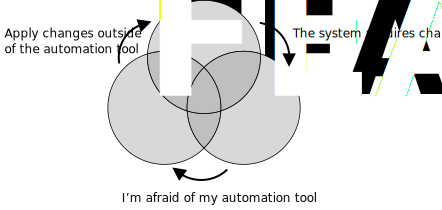
\includegraphics[scale=1]{images/automation-fear-spiral.pdf}
	\caption{Automation Fear Spiral}
	\label{fig:automation-fear-spiral}
\end{figure} 

Because of no trust for the automation, changes are applied manually to the systems and outside the defined automation process. If the system is reproduced, definitions may be missing in the templates, which leads to an inconsistent system. Therefore, enterprises have to break this spiral to fully profit from IaC \cite{Morris2016}. \\

When enterprises have moved their legacy systems to IaC, they can not only manage their systems faster, they also can profit from the principles of IaC as discussed in Section \ref{sec:iac-principles}. With IaC, systems are less complicated to manage, changes can be applied without fear, and the systems can easily be moved between environments. This provides the enterprises with more space to maneuver, systems can become more complex but still easy to manage, the systems can be defined and created faster which could lower costs.    

\section{Principles of Infrastructure as Code}
\label{sec:iac-principles}
The principles of IaC solve the problems of systems of the iron age. In the iron age the creation and maintenance of systems were a long, complicated and error prone process which consumed a lot of resources and time. With the decoupling of the physical hardware from the system, the creation and maintenance of the system has become simple, due to the IaC DSL and tooling. 

\subsection{Infrastructures are Reproducible}
\label{sec:iac-principles-reproducibility}
With IaC, systems are easy reproducible. It is possible to reproduce the whole infrastructure or parts of it effortlessly. Effortless means, that no tweaks have to be made to the templates or during the reproduction process and there is no need for a long term decision process about what has to be reproduced and how to reproduce it. To be able to reproduce system effortlessly is powerful, because it can be done automatically, consistently and with less risk of failures \cite{Morris2016}. The reproducibility of a system is based on reusable templates which provide the possibility to define parameters, which are set for the different environments as shown in Figure \ref{fig:reproduce-infrastructure}.

\begin{figure}[htbp]
	\centering
	\includegraphics[scale=0.95]{images/reproduce-infrastructure.pdf}
	\caption{Schema of a parametrized infrastructure deployment}
	\label{fig:reproduce-infrastructure}
\end{figure} 

\subsection{Infrastructures are Disposable}
\label{sec:iac-principles-disposable}
Another benefit of IaC is that systems are disposable. Disposable means, that systems can be easily destroyed and recreated. Changes made to the templates of a system does not have to be applied on an existing system, but can be applied by destroying and recreating the system. An requirement for a disposable system is, that it is understood that systems will always change. Other systems relying on a disposable system need to address that the system could change at any time. Systems must not fail because a disposable system disappears and reappears again because of an redeployment \cite{Morris2016}.

\subsection{Infrastructures are Consistent}
\label{sec:iac-principles-consistency}
Systems managed with IaC are consistent, because they are defined via a template and all instances are an instance of the template, with the little configuration differences defined by parameters. As long as the system changes are managed by IaC, the system will stay consistent, and the automation process can be trusted. \\

In Listing \vref{src:iac-template-docker-compose} an example for an IaC template is shown, which defines a Docker Compose service infrastructure for hosting a Wildfly server instance \cite{Wildfly2017, DockerCompose2018}. This system can consistently be reproduced on any environment supporting Docker, Docker Compose and providing values for the defined parameters. \\

\begin{code}
	\yamlFile{\sourceDir/iac-docker-compose.yml}
	\caption{Example for an IaC template for Docker Compose}
	\label{src:iac-template-docker-compose}
\end{code}

\subsection{Actions are Repeatable}
\label{sec:iac-principles-repeatability}
Building reproducible systems, means that any action applied to the system should be repeatable. Without repeatability, the automation cannot be trusted and systems wouldn't be reproducible. An instance of a system in another environment should be equal to any other system instance, except for the configurations defined by parameters. If this is not the case, then a system is not reproducible, because it will have become inconsistent \cite{Morris2016}. \\

IaC is a concept which makes it very easy to deal with systems in the cloud age. Enterprises can make use of IaC to move their legacy systems to the cloud, where they can profit from the principles of IaC. Nevertheless, before an enterprise can profit from IaC, it has to apply clear structures to their development process, as well as sticking to the principles of consistency and repeatability. For experienced administrators, who are used to maintain systems manually, it could sometimes be hard to understand why they are not supposed to perform any actions on the system manually anymore, nevertheless that a manual change could be performed faster. Being capable to reproduce a system at any time with no effort,  or applying changes on an existing system in a predefined and consistent manner,  makes enterprises very flexible and fast. Enterprises will not have to fear future changes in requirements and technologies of their systems anymore.    




\chapter{Containerization with Docker}
\label{cha:containerization-docker}

\section{The need for Containerization}
\label{sec:docker-containerization}

\section{Containerization Concepts}
\label{sec:docker-concepts}

\section{Virtualization vs. Containerization}
\label{sec:docker-virtualization-vs-containerization}
\chapter{Container as a Service with Kubernetes}
\label{cha:caas}
Container as a Service (CaaS) is a term introduced by cloud providers, which provide a cloud based on demand container environment. But CaaS is more then just an on demand container environment like Docker, it provides orchestration and monitoring tooling for containers, and additionally, CaaS is considered to be a model for IT organizations and developers how they can ship and run their applications anywhere. There are multiple CaaS providers on the market, but the most popular CaaS providers are Azure Container Service, Amazon Elastic Container Service for Kubernetes (Amazon EKS), and Google Kubernetes Engine, whereby they bring in their own flavor of CaaS, but all of them use Kubernetes beneath\cite{CNCFKubernetes2018, MicrosoftAzureAKS2018, AmazonWebServicesEKS2018, GoogleCloudKE2018}. \\

Kubernetes is a container orchestration platform for automating deployments, scaling, and operation of containers across a Kubernetes Cluster. Kubernetes has been invented by Google, is open source since 2015, and managed by the Cloud Native Computing Foundation (CNCF), whereby CNCF is under the umbrella of the Linux Foundation. Kubernetes has become the most popular container orchestration platform on the market and is used by many CaaS and PaaS providers\cite{CNCF2018}.

\section{The need for Container as a Service}
\label{sec:caas-need-for-caas}
Enterprises and developers face the need to dynamically adapt to workloads and to roll out new version of their services fast, and without any downtime. Applying dynamically to workloads requires a dynamic infrastructure, which is capable of scaling up, when the workload increases, and scaling down, when the workload decreases, which is non trivial to be handled manually. Rolling out new versions without downtime require a well defined workflow, which ensures a well defined roll out behavior. For such uses cases, a CaaS platform like Kubernetes can be used. Kubernetes makes it possible to effortlessly manage complex service infrastructures, service scaling, and the roll out of services. Thus, complex service infrastructures become simple to implement and manage. \\

Kubernetes provides a DSL, which allows to specify the desired state of the Kubernetes Cluster, as well as a automation tooling to interact with the Kubernetes Cluster. Kubernetes automatically ensures that the state of the Kubernetes Cluster meets its specification. Thus, the developers have only the need to specify the desired state of their Kubernetes Cluster. Kubernetes provides enterprises a platform for their services, which is effortlessly to specify and maintain via templates, and the provided automation tooling, which makes Kubernetes an IaC tool as well, as discussed in Chapter \vref{cha:iac}. This makes it easy to modify the infrastructure at any time, which allows enterprises to apply to new requirements fast.

\section{Kubernetes}
\label{sec:caas-kubernetes}
Kubernetes is a CaaS platform to orchestrate containers in a cluster, whereby the Kubernetes Cluster-Nodes can be located in the cloud or in a dedicated data center. Kubernetes is designed as a client server architecture and a master slave architecture. At least one node in the Kubernetes Cluster acts as the Kubernetes Master, which is discussed in Section \vref{sec:caas-kubernetes-master}, and the other nodes in the Kubernetes Cluster act as the Kubernetes Workers, which are discussed in Section \vref{sec:caas-kubernetes-worker}. The Figure \ref{fig:kubernetes-cluster-architecture} illustrates the architecture of a Kubernetes Cluster.

\begin{figure}[htbp]
	\centering
	\includegraphics[scale=1]{images/kubernetes-cluster-architecture.pdf}
	\caption{Architecture of a Kubernetes Cluster}
	\label{fig:kubernetes-cluster-architecture}
\end{figure} 

\subsection{Kubernetes Objects}
\label{sec:caas-kubernetes-objects}
Kubernetes Objects are persistent objects in the Kubernetes System, and the Kubernetes Objects describe the state of the Kubernetes Cluster. The Kubernetes Cluster ensures that the state of the cluster meets the state specified by the Kubernetes Objects. The developers don't have to manually perform actions in the Kubernetes Cluster, they just have to modify the state of the Kubernetes Objects, and the Kubernetes Clusters itself will ensure that the modified state is applied on the Kubernetes Cluster. The following sections will briefly introduce some of the common used Kubernetes Objects. The overview of all Kubernetes Objects is covered by the Kubernetes API reference documentation\cite{CNCFKubernetesAPI2018}. 

\mysubsubsection{Pod}
A Pod is a group of one or more containers, which are managed together, and therefore share the same life-cycle. A Pod specification contains the specification for each container in the group. All of the containers of a Pod are always scheduled on the same Kubernetes Worker-Node, and will be deployed, started and stopped, as a single unit. In a pre-container world, all of the applications represented by the containers would have been hosted on the same physical machine. A Pod allows to bundle containers together, whereby the containers in a single Pod represent one instance of one application\cite{CNCFKubernetesPods2018}. 

\mysubsubsection{Service}
A service is an abstraction, which defines a set of Pods and policies how to access them. The connection to the Pod, via the service abstraction, is handled by the Kubernetes Proxy. The service abstraction is necessary, because a Pod can be hosted on any Kubernetes Worker-Node within the Kubernetes Cluster, and the Pod will therefore get a random IP assigned, which makes it impossible to address the Pod directly. If multiple replicas of a Pod are running, then the service will load balance the request between the Pods of the replica set, depending on the chosen algorithm\cite{CNCFKubernetesServices2018}.

\mysubsubsection{Secret}
A secret is an abstraction to manage sensitive configuration data, which can be consumed by containers. A secret holds a set of key value pairs, which represents the sensitive configuration data, and can be referenced by its name. A referenced secret can be injected into the container, either as a environment variable, or a file, whereby the filename will represents the secret key and the file content represents the secret value. Developers reference secrets in the specifications by their name, and only the referencing containers can access the injected sensitive configuration data the secret holds\cite{CNCFKubernetesSecrets2018}. 

\mysubsubsection{ConfigMap}
A configuration map works the same way as secrets, but is intended to hold non sensitive configuration data\cite{CNCFKubernetesConfigMap2018}.

\subsection{Kubernetes Master}
\label{sec:caas-kubernetes-master}
The Kubernetes Master is the master node in the Kubernetes Cluster. It is responsible for managing the Kubernetes Worker-Nodes and containers running on those nodes. The Kubernetes Master exposes a REST API, via clients can interact with the cluster. The node hosting the Kubernetes Master should be exclusively for the Kubernetes Master. The following sections briefly introduce the Kubernetes Master-Components, which are responsible for managing the Kubernetes Cluster\cite{CNCFKubernetesComponents2018}.

\mysubsubsection{Kubernetes CLI (kubectl)}
Kubectl is the CLI of Kubernetes, which provides an interface to manage the Kubernetes Cluster, and to manage Pods running on the Kubernetes Worker-Nodes. Kubectl is similar to the Docker CLI, but does not support direct interacting with Docker. Kubectl interacts with the Kubernetes Cluster via the REST API exposed by the Kubernetes Master API-Server. Kubectl can be used from any client machine, which can connect to the cluster without any special setup.

\mysubsubsection{Distributed Key-Value Store (etcd)}
Etcd is a distributed key-value store, and provides a reliable way for sharing data within a cluster. It is the key component for the communication between the Kubernetes Master nodes and the Kubernetes Worker nodes. The Kubernetes Master provides configuration for the Kubernetes Worker nodes, and the Kubernetes Worker nodes provide state information for the Kubernetes Master nodes\cite{CoreOSETCD2018}.

\mysubsubsection{Kubernetes API-Server (kube-apiserver)}
The Kubernetes API-Server exposes the REST API for interacting with the Kubernetes Cluster, and is located on the Kubernetes Master. It represents the front-end of the Kubernetes Cluster and provides all necessary API to manage the Kubernetes Cluster, and the Kubernetes Objects.

\mysubsubsection{Kubernetes Scheduler (kube-scheduler)}
The Kubernetes Scheduler watches the Kubernetes Cluster for newly created Pods and assigns the Pods to a Kubernetes Worker-Node. The Kubernetes Scheduler decides which Kubernetes Worker-Node is suitable for the Pod. Multiple factors are taken into account for scheduling decisions such as, individual specifications, resource requirements, available resources, and hardware/policy/software constraints.

\mysubsubsection{Kubernetes Controller Manager (kube-controller-manager)}
The Kubernetes Controller Manager is responsible for managing the different controllers. A Kubernetes Controller is running in a loop and ensures that the state of the system is valid, depending on the controller type. For instance, the replication controller ensures the correct number of Pods, for each replication controller object  within the Kubernetes Cluster. Kubernetes provides a set of controllers such as a replication controller, node controller, endpoint controller, and service account controller.

\subsection{Kubernetes Worker}
\label{sec:caas-kubernetes-worker}
The Kubernetes Worker is a node within the Kubernetes Cluster, which acts as the slave node, which runs the Pods, and is managed by the Kubernetes Master. The Kubernetes Worker can be a VM or a physical machine, depending on the Kubernetes Cluster setup. It contains the Kubernetes Runtime-Environment and used container runtime. The following sections briefly introduce the Kubernetes Worker-Components, which are responsible for running the Pods on the Kubernetes Worker-Node\cite{CNCFKubernetesComponents2018}. 

\mysubsubsection{Kubernetes Agent (kubelet)}
The Kubernetes Agent is a process, running on the Kubernetes Worker-Node, which interacts with the Kubernetes Master via its exposed REST API. The Kubernetes Agent ensures that the containers are running in a Pod, as specified by the provided Pod specifications. The Pod specifications can be provided by an file in a specific directory (gets periodically checked), or via the Kubernetes API-Server.

\mysubsubsection{Kubernetes Network-Proxy (kube-proxy)}
The Kubernetes Network-Proxy manages the networks defined by the specifications, and reflects the services, which are bound to a Pod. It can perform simple TCP and UDP forwarding, and can be connected to multiple back-ends. Any communication of a Pod to another Pod or to an external network is handled by the Kubernetes Network-Proxy. 

\mysubsubsection{Container Runtime}
The container runtime is the software responsible for running the containers on the Kubernetes Worker. Kubernetes supports multiple container runtimes, but mostly  Docker is used, which has been discussed in Chapter \vref{cha:containerization-docker}. \\

Kubernetes provides all features to implement a dynamic scalable service infrastructure such as, workflows for rolling out services, replica management, or secret and configuration management. Kubernetes is on top of the container runtime such as Docker, and provides orchestration tooling, necessary to run large scale containerized service infrastructures. Nevertheless, sometimes a pure container orchestration platform like Kubernetes is not enough, which for instance provides no features for setting up a complete release workflow. This can be overcome with the usage of PaaS platforms like Openshift, which is discussed in the following chapter.

\chapter{Platform as a Service with Openshift}
\label{cha:paas}
Platform as a Service (PaaS) ...

\section{The need for Platform as a Service}
\label{sec:paas-need-for-paas}
As mentioned in Section \vref{sec:caas-kubernetes-worker}, there are some use cases where Kubernetes or in particular CaaS is not suitable anymore. CaaS is suitable if its used by developers, but not for persons without any deep knowledge of Docker and Kubernetes. This is where PaaS platforms come into place, which provide a web console and a template mechanism, which can be used by non-developers. Developers specify templates for the provided services which contains all technical parts of a service infrastructure and non-developers provide values for the exposed parameters which are non-technical, and the PaaS platform instantiates the template and deploys the service infrastructure automatically. \\

Enterprises can profit from PaaS platforms by defining templates for services they provide for their departments, partners or customers, who can create an instance of a provided service on demand, and destroy it if not needed anymore. PaaS platforms provide a self service console, where services can be created, managed and destroyed effortlessly without the need to understand the underlying technology. The self service console could be implemented by enterprises for their use cases, where the self service console interacts with PaaS via its exposed API. \\

PaaS platforms like Openshift usually provide an integration in a Continuous Integration / Continuous Deployment (CI/CD) workflow, which allows to automatically build and deploy new service releases on the PaaS platform automatically via web hooks. Therefore, the PaaS platforms are integrated in the whole software life cycle. This decreases the effort of the developers to interact with the cloud platform and provide additional automation.

\section{Openshift}
\label{sec:paas-kubernetes}
Openshift is a open source PaaS platform, which uses Docker and Kubernetes for the Docker Container orchestration. Openshift is designed as a client server architecture and a master slave architecture. One Openshift cluster can contain multiple Kubernetes clusters which are managed by the Openshift Master-Node which is discussed in Section \vref{sec:paas-openshift-master}. Openshift organizes the Kubernetes namespaces in so called projects, which place all defined resources in a Kubernetes namespace, and which are isolated form each other. Kubernetes organizes the resources in namespaces but does not provide any security mechanism for isolating those namespaces. Kubernetes also provides no monitoring tooling and web console for managing its resources. The Figure \vref{fig:paas-openshift-project-architecture} illustrates the Openshift Project-Architecture, its contained Openshift Objects, Kubernetes objects and their dependency to each other.

\begin{figure}[htbp]
	\centering
	\includegraphics[scale=1]{images/openshift-project-architecture.pdf}
	\caption{Architecture of a Openshift Project}
	\label{fig:paas-openshift-project-architecture}
\end{figure} 
The Openshift Objects, which are contained in an Openshift Project are briefly discussed in the following Section \vref{sec:paas-openshift-objects}.

\subsection{Openshift Objects}
\label{sec:paas-openshift-objects}
Openshift Objects are persistent objects in the Openshift System, and the Openshift Objects describe the state of the Openshift Cluster. This behavior has been inherited from the underlying used Kubernetes System as discussed in Section \vref{sec:caas-kubernetes-objects}. The following sections briefly introduce the Openshift Objects which enhance the Kubernetes System. 

\mysubsubsection{Build Configuration}
The Build Configuration specifies the way how a Docker Image is built on the Openshift platform. The built Docker Image is pushed the Openshift internal Docker Registry. Openshift Build Configurations support the following listed strategies \cite{OpenshiftBuildAndImageStreams2018, S2I2018}.
\begin{itemize}
	\item The \emph{Source-to-Image (S2I)} strategy is the build strategy which builds a Docker Image from source code.
	\item The \emph{Docker} strategy is the build strategy which builds a Docker Image from a Dockerfile.
	\item The \emph{Custom} strategy is the build strategy which build a Docker Image with a custom implemented build mechanism.
	\item The \emph{Pipeline} strategy is the build strategy which performs a Jenkins pipeline build on a Jenkins build server.
\end{itemize}
The necessary resources for the particular build strategy are provided via a git repository, and a Build Configuration can be triggered by an external service such as Github via a web hook. 

\mysubsubsection{Deployment Configuration}
A Deployment Configuration specifies how a deployment unit has to be performed. A Deployment Configuration allow to specify the Kubernetes life cycle hooks pre-hook or post-hook, which are used to configure the deployed Pod before its process has started (pre-hook) or after its process has started and is ready (post-hook). Deployment Configurations support the following deployment strategies.
\begin{itemize}
	\item The \emph{Rolling} strategy is the deployment strategy which waits for the new deployment to be ready before the old deployment gets removed.
	\item The \emph{Recreate} strategy is the deployment strategy which removes the old deployment when the new deployment gets started.
	\item The \emph{Custom} strategy is the deployment strategy which performs the deployment by a custom implementation.
\end{itemize}


\mysubsubsection{Route}
\mysubsubsection{Service}
\mysubsubsection{Docker Registry}

\newpage 

\subsection{Openshift and Kubernetes}
\label{sec:paas-openshift-and-kubernetes}

\begin{figure}[htbp]
	\centering
	\includegraphics[scale=1]{images/openshift-kubernetes-cluster-architecture.pdf}
	\caption{Architecture of a Openshift-Kubernetes Cluster}
	\label{fig:paas-openshift-kubernetes-cluster-architecture}
\end{figure} 


\subsection{Openshift Master}
\label{sec:paas-openshift-master}
\chapter{Enterprise Service Bus}
\label{cha:esb}
An Enterprise Service Bus (ESB) is a architectural pattern which describes a distributed computing architecture, whereby distributed services are interacting with each other via the ESB. The ESB pattern if part of the Service Oriented Architecture Patterns (SOA).   
\\ \\
An ESB in the industry is mostly taken as a third party middleware, which provides features for implementing integrations with the Enterprise Integration Patterns (EI). Enterprises use third party middleware like JBoss Fuse for implementing integration services, which integrate external or internal services. JBoss Fuse is based on the Enterprise Application Platform (EAP), and bundles common frameworks used for integrations such as Camel, and is responsible for orchestration and mediation of the services.
\\ \\
The integration of internal as well as external services has become more important over time, especially with the appearance of cloud platforms like PaaS. Common ESB middleware on the market usually define the ESB as a single application, which contains all integration services, whereby all integration services share the same life-cycle. But the need for flexibility and shorter response times drives enterprises to split up their teams and integrations. This leads to separated services, which are managed as microservices, which have their own life cycle. De-coupling of teams leads to de-coupling of services, where the services need to provide a well defined and well managed public API\cite{Camel2015, RedHatAgileIntegration2017, EIP}.

\section{The need for an Enterprise Service Bus}
\label{sec:esb-need-for-esb}
Enterprises need an ESB to provide integrations between internal and external services or both, where the integration is meant to provide a business value for the enterprise. An integration of an external service could enhance the reach of a customer, who now could be able to consume external partner services via the enterprise provided infrastructure or product. In the digital age, it is normal to consume a digital service like Netflix, which runs a streaming service. Thus, integrations an enterprise has to provide and maintain will become more over time.

\section{Architecture}
\label{sec:esb-architecture}
Figure \vref{fig:esb-simple-architecture} illustrates the conceptional architecture of an ESB, which orchestrates and mediates integration services. A service can act either a producer service, which gets accessed by clients, or can act as a consumer service, which acts as the client for a producer service. The ESB is responsible for orchestration, mediation, security, transformation, routing and service discovery, whereby these aspects are covered by a ESB middleware provided frameworks and libraries. Additionally, an ESB middleware provides libraries which help to implement Service Components under consideration of the SOA and EI Patterns\cite{EsbSoa2018, MediationESB2005}.

\begin{figure}[htbp]
	\centering
	\includegraphics[scale=1]{images/esb-simple-architecture.pdf}
	\caption{Architecture of an ESB}
	\label{fig:esb-simple-architecture}
\end{figure} 

\begin{figure}[htbp]
	\centering
	\includegraphics[scale=1]{images/esb-bidirectional-integration.pdf}
	\caption{Architecture of a bi-directional enterprise integration}
	\label{fig:esb-bidirectional-integration}
\end{figure} 

Figure \vref{fig:esb-bidirectional-integration} illustrates a bi-directional integration of services between two partner enterprises, whereby each integrated service is allowed to be consumed by the partner's customers, but only if the service is accessed via the partner's infrastructure. The ESB of the enterprises integrate the partner's provided services into their service domain, which can be accessed by their customers. For instance, an IP-TV provider can be integrated by an Internet Service-Provider (ISP), to provide Internet TV to their customers. 

\section{ESB with EAP}
\label{sec:esb-as-software}
An ESB is an architectural pattern for a distributed system, and has been implemented in software to provide an integration platform to developers, so that they can implement services under the consideration of the EAI patterns. Before the appearance of cloud platforms like PaaS, ESB implementations used existing platforms such as JBoss EAP, OSGI or Karaf for the service orchestration and mediation. In case of JBoss EAP, the platform provides all libraries and frameworks developers need for implementing a service. Commonly, the services are managed within a single application, which represents ESB. This is a monolithic approach of organizing services, but has the advantage that the management of the services is easier, because the source code is not separated, and therefore the implementations of all services needs to be consistent at compile time. Figure \vref{fig:esb-software-architecture} illustrates the monolithic organization of the services within a single ESB application, which is hosted on JBoss EAP.

\begin{figure}[htbp]
	\centering
	\includegraphics[scale=1]{images/esb-software-architecture.pdf}
	\caption{ESB running on EAP}
	\label{fig:esb-software-architecture}
\end{figure} 

With the appearance of cloud platforms such as PaaS, the cloud can now take over the mediation, orchestration and security aspects of an ESB. The integration services can be completely separated and de-coupled from each other, designed as microservices with their own life-cycle, and be managed by the cloud platform. Additionally, the integration services are hosted in a clustered infrastructure, which allows them to be distributed among multiple nodes, which increases fail over security. The new term for this kind of ESB is IPaaS, whereby the ESB is represented by an PaaS platform such as Openshift, which provides additional tooling for implementing integration services\cite{iPaaSP12015, iPaaSP22015}.

\section{ESB with Openshift}
\label{sec:esb-as-cloud}
With the appearance and general availability of cloud platforms like PaaS, it is possible now to move an ESB into the cloud, whereby the cloud platform takes over some aspects of the ESB middleware such as mediation and orchestration. A main problem of existing ESB implementations is the fact, that all integration services are managed within a single application, with one release version, and a shared life-cycle. If the ESB is an cloud platform, the integration services have to be implemented as separated services, which forces developers to separate their integration services into separate code bases, and to provide a proper designed and managed public API for their services. Figure \vref{fig:esb-cloud-architecture} illustrates the integration services of an ESB application, which runs on Openshift.

\begin{figure}[htbp]
	\centering
	\includegraphics[scale=1]{images/esb-cloud-architecture.pdf}
	\caption{ESB application architecture with microservices}
	\label{fig:esb-cloud-architecture}
\end{figure} 

As discussed in the introduction of this chapter, enterprises need to separate their integrations and teams, to be faster and more responsive to business changes. Therefore, the microservice architecture, which is necessary when the ESB is represented by a cloud platform, can help enterprises to become more flexible.

\section{Integration example}
\label{sec:esb-integration-example}
This section will discuss an integration examples, and how it would have been designed as part of a monolithic ESB application. The integration discussed in this chapter is the base for the prototype of this thesis, which is specified in Chapter \vref{cha:esboc}. Figure \vref{fig:esb-design-services} illustrates the integration example, contained services and involved service domains. The integration service integrates an external database with an internal application, which is consumed by a public client. How the database is allowed to be accessed, is implemented in the integration service, which is the only service allowed to communicate with the external located database.
\newpage

\begin{figure}[htbp]
	\centering
	\includegraphics[scale=1]{images/esb-integration-example.pdf}
	\caption{Integration Service-Domains}
	\label{fig:esb-design-services}
\end{figure}

Figure \vref{fig:esb-design-sca} illustrates the design of the integration in an monolithic ESB application, with the use of Service Component Architecture (SCA). A service within the ESB application is represented by a service component, which exposes consumable services (\mentionedtext{Service}) and is connected to other services or external systems (\mentionedtext{Reference}). 

\begin{figure}[htbp]
	\centering
	\includegraphics[scale=1]{images/esb-sca-example.pdf}
	\caption{Integration Services with SCA}
	\label{fig:esb-design-sca}
\end{figure}
  
ESB middleware, such as JBoss Fuse provides frameworks and libraries, which implement the SCA patterns and provide a lightweight way of implementing service components. The service component orchestration, mediation is done by the ESB middleware. Additionally, the ESB middleware provides bindings for commonly used technologies such as REST or SOAP, which can be applied to services and references. Thus, the developers don't have to setup for instance a REST Server or REST Client anymore, but only need to provide the service contract and connection settings\cite{MicroSoa2008, Richards2015}.\\

The following chapter will specify the prototype based on the introduced integration example, and will show that an ESB can be implemented on Openshift.
\chapter{Design ESB in Openshift}
\label{cha:esboc}
In this chapter, the ESB example integration of Section \vref{sec:esb-integration-example} will be designed as microservices, which can run on a Openshift Cluster. An Openshift Project will act as the ESB, which will provide the mediation, security, configurations and secrets for the services. The concrete functionality of the services is considered to be not important. The goal is to redesign the service components of Figure \vref{fig:esb-design-sca} as microservices, and to design the Openshift Project, which will host the services and act as the ESB. \\

As discussed in Chapter \vref{cha:esb}, an ESB is a distributed architectural model, whereby services act as a consumer or producer. These services provide a business value for an enterprise in form of an integration of an internal or external service. There are multiple providers of ESB middleware like JBoss Fuse, which provide tooling for implementing service components running on the ESB middleware. The prototype will illustrate that SOA service components can be implemented as microservices, whereby features provided by the ESB middleware, such as bindings, will have to be replaced by other implementations.

\section{Microservice Architecture}
Figure \vref{fig:esboc-design-services} illustrates the microservice architecture of the example integration of Figure \vref{fig:esb-design-sca}. Conceptually, the transformation of a service component to a microservice is easy, because a service component and a microservice act very similar. Compared to a service component of an ESB middleware, a microservice is completely separated from the other services, brings in its own libraries, and runs in its own runtime environment. From the implementation point of view, the microservices need to provide an runtime environment, which was previously provided by the ESB middleware. Therefore, that the microservices are completely separated, the access of other services is not mediated as usual anymore, because the communication is now performed via standard protocols like HTTP(S). In a monolithic ESB application, running on JBoss EAP, every service component is accessed via a reference, whereby the reference proxies the request directly to the service, which is running in the same runtime environment. With microservices, running in their own runtime environment, it is not possible to access the service instance directly anymore. Only communication via standard protocols, such as HTTP(S), is supported.

\begin{figure}[htbp]
	\centering
	\includegraphics[scale=1]{images/esboc-design-microservice.pdf}
	\caption{Integration with microservices}
	\label{fig:esboc-design-services}
\end{figure}

\section{Microservice Aspects}
\label{sec:esboc-aspects}
This section will discuss the necessary aspects of microservices, which will ensure, that the services are properly implemented, and can effortlessly be managed. Especially the monitoring of the services becomes very important, when moving from a conventional monolithic ESB application, like an application running on JBoss Fuse, to a microservice architecture based ESB application. Services running as microservices on Openshift, are running in their own runtime environment, and therefore cannot share any runtime resources. \\

Figure \vref{fig:esboc-aspects} illustrates the hierarchy of the microservice aspects, which will ensure that the implemented services are
\begin{itemize}
	\item secure,
	\item configurable for multiple environments,
	\item observable by developers and operators,
	\item resilient to failures
	\item and measurable.
\end{itemize}

The prototype will be implemented in Java, whereby the Eclipse community has provided the MicroProfile specifications, which provide an API to cover most of the microservice aspects. Using the MicroProfile specifications decreases the implementation effort, and provides a standardized way to implement microservices\cite{EclipseMicroprofileCharter2017}. \\

The following sections will specify the microservice aspects for the to implement microservices. 
\newpage

\begin{figure}[htbp]
	\centering
	\includegraphics[scale=1]{images/esboc-requirement-services.pdf}
	\caption{Microservice aspects}
	\label{fig:esboc-aspects}
\end{figure} 

\subsection{Security}
\label{sec:esboc-aspects-security}
Distributed services need to be secured properly from unauthorized access, therefore the microservices will be secured with OAuth2. OAuth2 is a token based authentication scheme, which has become popular over past few years. There are several open source implementations for interacting with an authentication service via the OAuth2 scheme. The Integration Service must authenticate its client, the Application Service, against a central authentication service, whereby the Application Service will retrieve the access tokens from the central authentication service, and the Integration Service validates the provided token against the central authentication service\cite{OAuth2018}.

\subsection{Configuration}
\label{sec:esboc-aspects-config}
The Eclipse MicroProfile specifications provide the MicroProfile-Config specification, which provides an API to inject configuration parameters into CDI Beans. The injected configuration parameters are loaded from so called configuration sources. A configuration source can either be Java system properties, environment variables, properties files, YAML files, or custom implementations, for instance to retrieve configurations from a database. The services must be implemented in a way, to be configurable for different stages such as DEV (development) and PROD (production), whereby  the services are only allowed to use configuration parameters via injection\cite{EclipseMicroprofileConfig2018}.

\subsection{Tracing}
\label{sec:esboc-aspects-tracing}
The Eclipse MicroProfile specifications provide the MicroProfile-OpenTracing specification, which provides an API for tracing an application on a method level and across service boundaries. Distributed tracing allows to comprehend service or method call chains of distributed services. There is open source tooling available to analyze the collected tracing data, provided by the distributed services. The services must collect reasonable tracing information and send this data to a central tracing service\cite{CNCFOpentracing2018}.

\subsection{Logging}
\label{sec:esboc-aspects-logging}
Distributed logging allows to comprehend logs across service boundaries within a service call chain, whereby the logs of all involved services have to be marked with the same transaction id. There is open source tooling available to analyze the collected logs, provided by the distributed services. The services must provide all of their logging to a central service, whereby the logs must be marked with a transaction id, which is provided by the MicroProfile-OpenTracing-API. Optionally, the services are allowed to add additional markers, which can help developers and operators to analyze problems or to group service logs.

\subsection{Metrics}
\label{sec:esboc-aspects-metrics}
The Eclipse MicroProfile specifications provide the MicroProfile-Metric specification, which provides an API to define and manage metrics. Metrics allow to comprehend the state of a microservice, such as resource consumption, API calls, or failure counts. Metrics along with distributed tracing and distributed logging, provide the necessary data, developers and operators need to analyze failures in services, which occurred in service call chains. The services must collect reasonable metrics and publish those metrics, which can be made available to a central metric service\cite{EclipseMicroprofileMetrics2018}.

\subsection{Fault Tolerance}
\label{sec:esboc-requirements-service-fault}
The Eclipse MicroProfile specifications provide the MicroProfile-FaultTolerance specification, which provides an API to define fault tolerance behavior such as retries, timeouts, and error fall-backs. The fault tolerance of a service means, that if a depending service is not accessible at the time, a service must not fail immediately after the first try, but the service should retry to call the depending service for several times, and fail when all retries have failed. Such a behavior ensures, that short timed communication errors, redeployments, or overloads do not immediately cause a service to fail. The services must provide proper fault tolerance configuration and fall-back behavior, to be able to recover from such errors in a proper manner\cite{EclipseMicroprofileFault2018}.   

\subsection{API Management}
\label{sec:esboc-requirements-service-api}
The API management of a public API such as REST API and REST Models ensure, that the clients, using the public API, are not broken by changes, made on that API. There are several opinions on how API management can be done. A public API has to be stable per design, and needs to evolve and provide backward compatibility in a way, so that clients have enough time to catch up with the changes. Swagger has become very popular for documenting an API, whereby the documentation can be used to generate clients, provide documentation for developers and to test the public API. The services must be capable of migrating their public API in a way, that the clients are not broken by made changes. The services must provide a Swagger Documentation, and provide a capability to access the Swagger Documentation\cite{SmartBearSwagger2018, RestVersion2018}.

\section{Openshift Architecture}
\label{sec:esboc-design-oc}
Figure \vref{fig:esboc-design-openshift-project} illustrates the design of the Openshift Project, which will act as the ESB. As discussed in Section \vref{sec:paas-openshift-project}, Openshift isolates Kubernetes Namespaces  by bringing in the concept of an Openshift Project. Services in an Openshift Project, which are not exposed via an Openshift Route, are implicitly protected from access from external networks and other Openshift Projects. The Openshift Project will contain the Application Service, the Database Service and the Integration Service. The Application Service has access to the Internet, and will be accessed by the Client from the Internet via its public address. The Integration Service and the Database Service are not exposed to the Internet, and can only be accessed within the Openshift Project by their service names.

\begin{figure}[htbp]
	\centering
	\includegraphics[scale=1]{images/esboc-design-openshift.pdf}
	\caption{Openshift Project architecture}
	\label{fig:esboc-design-openshift-project}
\end{figure} 

All services provide their tracing and logging data to external services, whereby no special configuration will be needed in Openshift, because Openshift allows services to access external networks. The mediation of the services is managed by Kubernetes Services, whereby the services communicate with each other via their service names, which ensures, that the communication stays within the Openshift Project. The Openshift Project must manage all configurations and secrets, which can be referenced by the services.

\section{Openshift Requirements}
\label{sec:esboc-requirements-oc}
The implementation of the Openshift Project such as templates and scripts, must be implemented under consideration of the principles of IaC, which have been discussed in Section \vref{sec:iac-principles}. Sticking to the principles of IaC will ensure, that the Openshift Project can effortlessly be managed and reproduced on any Openshift Cluster. \\

The Openshift Project will host the services and manage their configurations and secrets via Openshift ConfigMaps and Openshift Secrets, which have been discussed in Section \vref{sec:caas-kubernetes-objects}. The configurations and secrets are managed outside the service code bases, and are provided by the Openshift Project for a specific stage, the Openshift Project represents. The configurations and secrets are supposed to be managed by operators, and are only made available to the services during runtime, and shouldn't be accessible by developers. \\

The services must manage their integration into Openshift, by providing the necessary templates, whereby configurations and secrets are referenced by their predefined names. The services must expose all necessary configuration parameters, which allow to configure the service for a specific stage, whereby the Openshift Project will provide the proper configuration and secret values for the specific stage. \\

The implemented prototype will consist of two Openshift Projects, whereby one Openshift Project will host the tracing service, log aggregation service and authentication service, and the second Openshift project will host the ESB services along with the simulated external database, which will be integrated. \\

The following chapter will discuss the implementation of the designed prototype. 

\chapter{Implementation ESB in Openshift}
\label{cha:esbi}

\section{JBoss Fuse Integration Services}
\label{sec:esbi-fis}

\section{Additional Monitoring Tooling}
\label{sec:esbi-additional-tooling}

\section{Implementation Microservice Architecture}
\label{sec:esbi-impl-services}
 which can be achieved with the framework Wildfly-Swarm. Wildfy-Swarm is the Java Enterprise answer to Spring Boot, where a Java Application Server is bootstrapped programmatically, which only contains the minimal set of dependencies referenced by the service. 

\subsection{Distributed Tracing}
\label{sec:esbi-impl-tracing}

\subsection{Distributed Logging}
\label{sec:esbi-impl-logging}

\subsection{API Management}
\label{sec:esboc-impl-api}

\section{Implementation Openshift Architecture}
\label{sec:esbi-impl-oc}

\subsection{Security}
\label{sec:esboc-impl-security}

\chapter{Discussion ESB in Openshift}
\label{cha:esbd}
This chapter will discuss the implemented prototype of Chapter \vref{cha:esbi}, and will discuss some important tasks such as 
\begin{itemize}
	\item managing multiple environments,
	\item managing service security,
	\item managing multiple service versions,
	\item managing public API migration,
	\item and managing Adapters and Message Translators as services,
\end{itemize}
which are very important, when running an ESB on Openshift. Whenever possible, Openshift will be compared to JBoss EAP, which can be used as the platform for the ESB middleware JBoss Fuse, as discussed in Section \vref{fig:esb-software-architecture}. \\

The prototype implementation represents an ESB running on Openshift, but is actually nothing more than an application represented by several microservices, running on a PaaS platform. Instead of managing a monolithic ESB application, as discussed in Section \vref{sec:esb-as-software}, the ESB application is split into independent microservices, which are managed completely separately. Because of the usage of Openshift as the platform, the implemented services of the prototype are distributed services per default, which is the nature of Kubernetes, which is the base for Openshift. Openshift takes care of the distribution of the Pods within the Openshift Cluster, and ensures, that the Pods are accessible via their related service abstraction. \\

When splitting any monolithic application into independent microservices, then the sum of resources needed by all microservices of the ESB, will be higher as the resources needed by a monolithic ESB. With microservices more resources are needed, due to the fact, that each microservice brings in its own runtime environment, whereby the monolithic ESB runs in one runtime environment. This a trade off, which needs to be considered when designing microservices for an ESB, or when splitting up a monolithic application to a microservice architecture. \\

Table \vref{tab:esbd-resource-monolith-vs-microservice} illustrates not a real world example, but shows the trend of the resource need of the whole application, when a monolithic application is split up into microservices. When the application is split up into too many microservices, then the needed resources increase drastically. The illustrated resources for the microservices are representing the minimum assigned resources the platform has to provide, to ensure, that all microservices will have the assigned resources available when they are under load.

{\renewcommand{\arraystretch}{1.2}%
\newcolumntype{m}{>{\hsize=.3\hsize}X}%
	\begin{table}[h]
		\begin{tabularx}{\textwidth}{ m|c|c|c|c }	
			\textbf{Resource}    & \textbf{Monolith} & \textbf{1 Micros.} & \textbf{10 Micros.} & \textbf{20 Micros.} \\  \hline
			\textit{$CPU/Cores$} & 2                 & 0.5                & 5                   & 10 \\
			\textit{$RAM/GB$}    & 3                 & 0.5                & 5                   & 10 \\ \hline
		\end{tabularx}
		\caption{Resource comparison of monolith and microservices}
		\label{tab:esbd-resource-monolith-vs-microservice}
\end{table}}

\section{Service mediation}
\label{sec:esbd-service-mediation}
The SOA Patterns specify a mediation layer as layer, which facilitates the communication across multiple services by providing an abstraction layer, which decouples the services from each other. The mediation layer ensures, that services can seamlessly communicate with replaced, relocated, or newly released services instances. Kubernetes provides the concept of a Kubernetes Service, which mediates the requests among multiple service instances represented by the service Pods. The Kubernetes Service is a content unaware mediator, because the message remains unchanged, and only mediation between service instances is supported.

\begin{figure}[htbp]
	\centering
	\includegraphics[scale=1]{images/esbd-service-mediation.pdf}
	\caption{Openshift Service mediation}
	\label{fig:esbd-service-mediation}
\end{figure}

Figure \vref{fig:esbd-service-mediation} illustrates a scenario, where the service Pod 2 on Node 2 fails, and gets recreated on Node 3, whereby it gets a new IP address assigned. The Kubernetes Service is aware, that Pod 2 has been recreated on Node 3, and will balance the requests to the recreated Pod 2 located on Node 3, when Pod 2 is fully up and running. A Kubernetes Service performs a simple mediation by abstracting service Pods via service names, and load balancing of the requests to the service Pods depending on the chosen algorithm. \\

With an ESB, there is no central mediator needed, because an ESB is a distributed architectural model, which has no central component like a Hub and Spoke architecture. If message translation is needed, because of a consumer incapability of supporting the ESB used message format and protocols, then an adapter and message translator is needed, as discussed in Section \vref{sec:esbd-adap-trans-service}. \\

The following sections will discuss the tasks introduced in the beginning of this chapter, and will show, that these task can be performed on the implemented prototype.

\section{Managing Multiple Environments}
\label{sec:esbd-multiple-env}
An ESB is commonly hosted on multiple environments, whereby at least one productive and one testing environment should be present. These environments were commonly a VM, which provided the runtime environment for the ESB middleware. As the prototype shows, the environment is now represented by an Openshift Project, which can be reproduced via scripts as discussed in Section \vref{sec:esbi-openshift}. \\

The services hosted on the ESB are using Fuse Integration Service 2.0 and its provided tooling, which ensure, that the services are properly encapsulated in a container, and are properly managed in Openshift. Therefore, the service developers provide the necessary Openshift Templates, which has the effect, that the operators have no interaction with the service artifacts and service runtime environments anymore. Operators have to manage
\begin{itemize}
	\item the Openshift Project, which contains the services,
	\item the Openshift ConfigMaps, which hold the service non-sensitive configuration,
	\item and the Openshift Secrets, which hold the sensitive service configuration.
\end{itemize} 
\ \\
Figure \vref{fig:esbd-multi-stage-env} illustrates the management and provisioning of multiple environments for an ESB, whereby the environment is represented by an Openshift Project. The Management Server pulls the scripts and Openshift Templates from a VCS Server, and the configurations from a Configuration Server, and uses them to provision new Openshift Projects, or manage existing ones. The scripts and Openshift Templates are separated from the configurations, which are providing the values for the scripts and Openshift Template-Parameters. With such an approach, the infrastructure becomes reproducible, versioned, and therefore consistent and disposable. These characteristics of IaC have been discussed in Chapter \vref{cha:iac}.
\newpage 

\begin{figure}
	\centering
	\includegraphics[scale=1]{images/esbd-multi-stage-env.pdf}
	\caption{Management and provisioning of multiple environments}
	\label{fig:esbd-multi-stage-env}
\end{figure}

The interaction of the Management Server, VCS Server and Configuration Server, as illustrated in Figure \vref{fig:esbd-multi-stage-env}, is similar to the Figure \vref{fig:reproduce-infrastructure}, which illustrated how a system can be reproduced with parametrized templates and an IaC tool. The Openshift CLI provides functionality to manage Openshift Objects, which is what needs to be done, when providing an environment in form of an Openshift Project.  \\

Table \vref{tab:esbd-multi-stage-env} compares the Openshift and JBoss EAP contained mechanisms, which provide the listed infrastructure features. As illustrated in the table, Openshift provides networking and isolation features, which are provided to JBoss EAP by its hosting environment such as a VM. Except of the networking and isolation feature, JBoss EAP supports all other features either natively or by supporting a third party library. Nevertheless, Openshift combines all features in one platform, and makes them manageable via Openshift Templates and the Openshift CLI. \\

Openshift runs Docker Containers, and therefore the programming language, the service was implemented with, doesn't matter, as long as the services can run in a container. Also, services hosted on PaaS platforms communicate via standard Protocols such as HTTP, which is commonly supported by almost any programming language. JBoss EAP on the contrary, runs only Java applications.
\newpage

{\renewcommand{\arraystretch}{1.2}%
\begin{table}[h]
	\begin{tabularx}{\textwidth}{ X|X|X }	
	  \textbf{Feature}                  & \textbf{Openshift}         & \textbf{JBoss EAP} \\  \hline
	  \textit{Staging}                  & Openshift Project          & Server Instance \\  \hline
	  \textit{Management}               & Openshift CLI              & JBoss CLI \\
	                                    & Openshift Web-Console      & JBoss Web-Console \\
	                                    & Openshift REST-API         & \\  \hline
	  \textit{Networking}               & Openshift Project          & None (external) \\
	                                    & Openshift Service          & \\  
	                                    & Openshift Route            & \\  
	                                    & Openshift Router           & \\  \hline
	  \textit{Isolation}                & Openshift Project          & None (external) \\  \hline
	  \textit{Configuration/Secrets}    & Openshift ConfigMaps       & Java System-Properties  \\
	                                    & Openshift Secrets          & Environment Variables \\
	                                                                && Password Vault \\  \hline
	  \textit{Service Distribution}     & Openshift Worker-Node      & Single JVM \\ 
			                                                        && Karaf \\  
			                                                        && OSGI \\  \hline
	  \textit{Service Roll-out}         & Recreate                   & Framework dependent, \\ 
			                            & Rolling                    & normally recreate \\ \hline
	  \textit{Language Support}         & All runnable in containers & Java \\
	\end{tabularx}
	\caption{Infrastructure feature comparison}
	\label{tab:esbd-multi-stage-env}
\end{table}}

The next section will discuss the service security within an Openshift Project, which can be managed the same way, as discussed in this section. Additionally to the security, provided by the isolation feature of an Openshift Project, the Management Server of Figure \vref{fig:esbd-multi-stage-env} could also manage custom security configurations, which can be managed via the Openshift CLI as well. 

\section{Managing Service Security}
\label{sec:esbd-service-security}
With a common ESB middleware, the services are protected by running within a single runtime environment, or by security features provided by a supported third party library. In an Openshift Project, the services are implicitly protected by being isolated in a Kubernetes Namespace, as discussed in Section \vref{sec:paas-openshift-project}, whereby the namespace of an Openshift Project cannot be accessed by other Openshift Projects without additional configuration. Services, which are supposed to be accessible from external networks, have to be explicitly exposed via an Openshift Route, which can handle secured connections, similar to an reverse proxy.
\newpage

\begin{figure}[htbp]
	\centering
	\includegraphics[scale=1]{images/esbd-service-security.pdf}
	\caption{Service security in an Openshift Project}
	\label{fig:esbd-service-security}
\end{figure}
\ \\
Figure \vref{fig:esbd-service-security} illustrates an example, similar to the implemented prototype, whereby two Openshift Projects host the same services, and where the Pod Networks of the two Openshift Projects are joined. The joined Pod Networks allow services hosted in project PROJ\_PROD\_2 to access services hosted in project PROJ\_PROD\_1 by their fully qualified service name. The fully qualified service name has the form of \mentionedtext{<service>.<project\_namespace>.svc.cluster.local}. Joining two Pod Networks is performed by Openshift Cluster administrators, and cannot be performed by developers. \\

Additionally to the isolation of the services within the Openshift Project, the Integration Service is secured via OAuth2, whereby the resource access is controlled by a central Authentication Server. On the one hand, the services are isolated within a Kubernetes Namespace, and on the other hand, additional security, such as access control, has to be provided by the service itself, because Openshift doesn't provide such a feature. It is not meant to isolate services from each other within an Openshift Project, because an Openshift Project, in particular a Kubernetes Namespace, should only contain a set of services, which don't have to be isolated from each other. \\
\newpage

Table \vref{tab:esbd-service-security} compares the Openshift and JBoss EAP contained mechanisms, which provide the listed security features. As illustrated in the table, Openshift doesn't provide any support for access control on the service level, which is normal for a PaaS platform, such as Openshift. The services, running in Docker Containers on an Openshift Cluster, have to implement access control, or have to use third party frameworks, such as the Keycloak Adapter, which provides access control features as discussed in Section \vref{sec:esbi-security}. JBoss EAP on the other hand is a Java Application-Platform, which provides support for access or user control for several providers. 

{\renewcommand{\arraystretch}{1.2}%
	\begin{table}[h]
		\begin{tabularx}{\textwidth}{ X|X|X }	
			\textbf{Feature}                 & \textbf{Openshift}      & \textbf{JBoss EAP} \\  \hline
			\textit{Network Isolation}       & Openshift Project       & None (VM) \\  \hline
			\textit{HTTPS}                   & Openshift Router        & Reverse Proxy \\
			                                 & Openshift Route         & Endpoint Configuration \\  \hline
            \textit{Access Control}          & None (external)         & Endpoint Configuration \\
                                                                      && Internal User-Database \\ 
                                                                      && External User-Database \\  \hline
            \textit{Single-Sign-On}          & None (external)         & Endpoint Configuration \\
                                                                      && Several SSO providers \\  \hline
		\end{tabularx}
		\caption{Security feature comparison}
		\label{tab:esbd-service-security}
\end{table}}

Openshift doesn't provide access control features to secure service resources, but provides security features such as user/group/role management, project permission management, Pod Network management, or quota management for Openshift Objects, such as Replication Controllers. Openshift uses Software Defined Networks (SDNs), whereby 
the services don't have to handle communication security, because the Openshift Cluster will take care of it. Exposed services are connected to an Openshift Route, whereby the Openshift Route, which acts as the reverse proxy, applies security to the communication on the external network. Within the isolated Pod Network, the services don't have to handle communication security, because this is handled by the Openshift Cluster. 

\section{Managing Multiple Service Versions}
\label{sec:esbd-multi-version-service}
Sometimes it is necessary to run multiple versions of a service, for instance, if a new version is released, or if a consumer is not capable of migrating to the new version, but provides a significant business value for the enterprise. Openshift provides mechanisms to run multiple versions of a service in several ways. Figure \vref{fig:esbd-service-multiple-versions} illustrates some scenarios for running multiple service versions on Openshift, whereby the illustrated scenarios of PROJ\_1 and PROJ\_2 are possible, because the old service version is N-1 compatible. N-1 compatibility means, that the service in the old version is capable of reading data written by the service in the new versions.
\newpage

\begin{figure}[htbp]
	\centering
	\includegraphics[scale=1]{images/esbd-service-multiple-versions.pdf}
	\caption{Running multiple service versions on Openshift}
	\label{fig:esbd-service-multiple-versions}
\end{figure}

\emph{PROJ\_1} of Figure \vref{fig:esbd-service-multiple-versions} illustrates an A/B Release, which is used to run the old and new version of a service in parallel, whereby a portion of the service consumers get access to the new version, while the rest of the service consumers are still using the old version. A/B Releases are used to validate the new version in the production environment, before fully releasing it to all consumers. In this scenario, the requests are load balanced by the Openshift Route to either the new or old service version. \\ 

\emph{PROJ\_2} of Figure \vref{fig:esbd-service-multiple-versions} illustrates a Blue/Green Release, which is used to run the old and the new version of a service in parallel, whereby the Openshift Route switches between the old and new service version. In this scenario, all service consumer access the same service version, which is currently accessible by the Openshift Route. \\

\emph{PROJ\_3} of Figure \vref{fig:esbd-service-multiple-versions} illustrates two service versions running completely separated in parallel, whereby both versions are accessible via their own Openshift Route. This scenario is not a release scenario, and should be used if multiple service versions have to be provided, for instance, if a customer cannot switch to the new version, but provides a significant business value to the enterprise. \\

Table \vref{tab:esbd-service-multiple-versions} compares the Openshift and JBoss EAP contained mechanisms, which provide the listed release features. Multiple service versions on an Openshift Cluster are represented by separate Openshift Service objects, whereby with JBoss EAP, multiple service versions are either represented by separate JBoss EAP instances, or deployment contexts on a single JBoss EAP instance. With JBoss EAP version switching and weighted routing can be performed by an external reverse proxy, which in Openshift can be performed by an Openshift Route.

{\renewcommand{\arraystretch}{1.2}%
 \newcolumntype{m}{>{\hsize=.32\hsize}X}%
	\begin{table}[h]
		\begin{tabularx}{\textwidth}{ X|X|X }	
			\textbf{Feature}                  & \textbf{Openshift}      & \textbf{JBoss EAP} \\  \hline
			\textit{Multiple Service Versions}& Openshift Service       & Multiple EAP instances \\
											  & Openshift Route    	    & Multiple deployment contexts \\ \hline
			\textit{Weighted Routing}         & Openshift Route         & None (external) \\  \hline
			\textit{Version Switch}           & Openshift Route         & None (external) \\  \hline
		\end{tabularx}
		\caption{Release feature comparison}
		\label{tab:esbd-service-multiple-versions}
\end{table}}

JBoss EAP is an application platform for Java applications, which provides a runtime environment for Java applications, but no networking features, as shown in Table \vref{tab:esbd-multi-stage-env}, and therefore no routing feature. JBoss EAP can be configured to act as a reverse proxy, but cannot act as the reverse proxy for applications hosted on the same JBoss EAP instance. As Figure \vref{fig:esbd-service-multiple-versions} illustrates, the implemented prototype can run multiple versions of the hosted services, and supports the implementation of release models such as A/B or Blue/Green Releases.

\section{Managing Migration of Public API}
\label{sec:esbd-multi-stage-env}
This section will discuss the management of services public API, which is crucial, when it comes to distributed services. Changes made on the public API of a service can break the functionality of an application, the service is part of, or break the functionality of an external application, which depends on this service. The public API is the API the service exposes, which could only be consumed by internal consumers, but has to be managed the same way, as the API would be exposed to external consumers. There are several ways to migrate a public API, whereby some of them will be discussed in the further sections. \\  

Services running on an Openshift Cluster are completely separated from each other and have their own life-cycle. Therefore, they have to provide a public API, which can be consumed by other services. The public API has to be designed properly in the first place, as well as the management of its migrations. At least, the last both versions will have to be supported, to give the developers of the consuming services enough time to apply to the migrations performed on the public API. Commonly, a service has two versions, the service release version, and the service API version, which is allowed to remain the same over multiple service releases. 
\newpage

The following sections will discuss the different ways to migrate the public API of a service.

\mysubsubsection{URL Query-Parameter Versioning}
Multiple versions of a public API can be managed via a URL Query-Parameter, whereby the URL Query-Parameter defines the version to use of a single API Operation. The URL \inlineBash{http://localhost/api/users?version=2} illustrates how to access a specific version of an API Operation via a URL Query-Parameter. Table \vref{tab:esbd-service-api-query-param} shows the Pros and Cons of API Versioning with URL Query-Parameters.

{\renewcommand{\arraystretch}{1.2}%
	\begin{table}[h]
		\begin{tabularx}{\textwidth}{ X|X }	
			\textbf{Pros}                 & \textbf{Cons}    \\  \hline
			Single resource address       & Data and control parameters are mixed  \\ \hline
			Supported by all browsers     & Version as data parameter not possible \\ \hline
			Easy to understand            & No declarative mapping with JAX-RS     \\ \hline
			Easy to implement             & Manual switch between API Operations   \\ \hline
		\end{tabularx}
		\caption{Pros and Cons of URL Query-Parameter Versioning}
		\label{tab:esbd-service-api-query-param}
\end{table}}

\mysubsubsection{HTTP Header Versioning}
Multiple version of a public API can be managed via HTTP Headers in the following listed ways:
\begin{itemize}
	\item New HTTP Header \\
	e.g. \inlineBash{Version: 2}
	\item Additional field in the Accept-Header \\
	e.g. \inlineBash{Accept: application/json; version=2}
	\item Enhanced Media-Type \\
	e.g. \inlineBash{Accept: application/vnd.app.model.v1+json;qs=0.9}
\end{itemize}
\ \\
The approach of HTTP Header Versioning brings in more flexibility, but also makes the API Versioning harder to understand for consumers, especially when quality of service is used in the HTTP Accept-Headers of multiple API Operations. Table \vref{tab:esbd-service-api-http-header} shows the Pros and Cons of API Versioning with HTTP Headers.

{\renewcommand{\arraystretch}{1.2}%
\begin{table}[h]
	\begin{tabularx}{\textwidth}{ X|X }	
		\textbf{Pros}                         & \textbf{Cons}                  \\ \hline
		Single resource address               & Header handling needed         \\ \hline  
		No mix of data and control parameters & Harder to understand           \\ \hline
		Declarative mapping with JAX-RS       & No enhanced Media-Type in HTML \\ \hline
		Easy to implement                     & More difficult to test         \\ \hline
	\end{tabularx}
	\caption{Pros and Cons of HTTP Header Versioning}
	\label{tab:esbd-service-api-http-header}
\end{table}}

\mysubsubsection{Path Versioning}
The easiest way to manage multiple versions of a public API is Path Versioning, whereby the whole API is versioned, instead of single API Operations. The URL \inlineBash{http://localhost/api/v2/users} illustrates how to access a specific version of an API Operation via a Path version. The Path Versioning is the most used approach to version a public API, because of its simplicity to realize.  Table \vref{tab:esbd-service-api-path} shows the Pros and Cons of API Versioning with Path versions.

{\renewcommand{\arraystretch}{1.2}%
	\begin{table}[h]
		\begin{tabularx}{\textwidth}{ X|X }	
			\textbf{Pros}                         & \textbf{Cons}                         \\ \hline
			Easy to implement                     & Multiple resource addresses           \\ \hline
			Easy to understand                    & Declarative mapping with JAX-RS       \\ \hline
			No mix of data and control parameters & Version actually not part of resource \\ \hline
			Easy to switch between versions       & Latest version unknown                \\ \hline
		\end{tabularx}
		\caption{Pros and Cons of Path Versioning}
		\label{tab:esbd-service-api-path}
\end{table}}

The prototype uses Swagger for documenting the services public API, as discussed in Section \vref{sec:esbi-api}, whereby Swagger is used to generate the Swagger Documentation and clients. One advantage of a Swagger generated client is, that developers work with generated classes and interfaces, and therefore, developers work with a typed client, which will cause compile errors on breaking API changes. The API changes can be performed in a way, whereby developers will not have to change anything in their source code, but could also be performed in a way to cause compile errors, which force the developers to apply to the breaking API changes. If the client is implemented by hand and not generated by a tool, then developers will have to ensure that the implemented client is in sync with the currently used API version.

\section{Managing Adapters and Message Translator as Services}
\label{sec:esbd-adap-trans-service}
Adapters and Transformers are part of the EI Patterns, whereby the Adapter is used to couple an application to a message bus, and the Transformer is used to transform messages from the application supported format to the message bus supported format and vice versa. The Adapter and Message Translator can either be  located at the external service, or can be located in the messaging system, the external service connects to. Commonly, a message bus system is implemented to use one form of communication, such as REST, and one form of data representation. If external services need to access the message bus, but don't support the message bus protocol and data format, then Adapters and Message Translators are needed, to connect the external service to the message bus. \\

Figure \vref{fig:esbd-service-adapter} illustrates how the prototype could be integrated with external applications via an Adapter and Message Translator. If the Adapter and Message Translator are located at the external service, then the Adapter and Message Translator have to be provided in the programming languages, the external services are implemented with. If the Adapter and Message Translator are located in the Openshift Project, then they can be implemented in the programming language of choice.

\begin{figure}[htbp]
	\centering
	\includegraphics[scale=1]{images/esbd-service-adapter.pdf}
	\caption{External services integrated via an adapter}
	\label{fig:esbd-service-adapter}
\end{figure}

The Adapter and Message Translator have to be implemented as a standalone application (microservice), which for instance can be realized in Java with the Camel framework, which provides an API for implementing EI Patterns, and is capable of running as a standalone application. The adapter and message translator application can be hosted as a separate Openshift Service, or can be added to the service Pod as a so called side-by container, which proxies the requests to the actual container.  \\

\section{Further Work}
\label{sec:esbd-furhter-work}
During writing this thesis and the implementation of the prototype, Red Hat has released its new version of the JBoss Fuse platform, which now is based on Openshift, and is called Red Hat Fuse 7. Red Hat Fuse 7 enhances Openshift with features for implementing an ESB, whereby the main goal is to provide non-technical personal the possibility to create integrations. Red Hat Fuse 7 provides IPaaS features, by providing a low/no code UI, which allows to create integrations without the need to write a single line of code. \\

The next step is to implement an ESB with Red Hat Fuse 7, to see the differences between the manual approach, represented by the prototype, and the approach using IPaaS provided features. Red Hat Fuse 7 should make it easier for enterprises to create integrations to external services, as well as the management of these integrations.   

%%%----------------------------------------------------------
\appendix                                         % appendix 
%%%----------------------------------------------------------

%\include{back/appendix_a}	% technical supplements
%\include{back/appendix_b}	% contents of the CD-ROM/DVD
%\include{back/appendix_c}	% chronological list of changes
%\include{back/appendix_d}	% source text of this document

%%%----------------------------------------------------------
\MakeBibliography                     				% references
%%%----------------------------------------------------------
%%% special page for checking print size --------------------
%\include{back/printbox}

%%%----------------------------------------------------------
\end{document}
%%%----------------------------------------------------------